\documentclass[11pt]{article}
\usepackage[margin=2cm, a3paper]{geometry}                % See geometry.pdf to learn the layout options. There are lots.
%\geometry{a3paper}                   % ... or letterpaper or a4paper or a5paper or ... 
%\geometry{landscape}                % Activate for for rotated page geometry
\usepackage[usenames,dvipsnames,svgnames,table]{xcolor}
\usepackage{tikz}
\usepackage[nonumberlist]{glossaries}
\usepackage{amsmath, amssymb}
\usetikzlibrary{mindmap}
\makenoidxglossaries

\newglossaryentry{tmp}{name={tmp}, description={}}

\newglossaryentry{monomial}{name={monomial}, description={Term of the form $a_{mn}x^my^n$ where $m,n$ are non-negative integers and $a_{mn}$ is arbitrary (Courant and John)}}
\newglossaryentry{tangent}{name={tangent}, description={A tangent line to a function $f(x)$ at a point $a$ has equation $y = f(a) + (x-a)f'(a)$.  A tangent plane to a function
$f(x,y)$ at a point $(a,b)$ has equation $z = f(a,b) + (x-a)f_x(a,b) + (y-a)f_y(a,b)$.  The tangent is a linear function with matching position and slope to the original function at the point of tangency (Wolfram MathWorld)}}
\newglossaryentry{directional derivative}{name={directional derivative}, description={The \emph{derivative in the direction $\vec{v}$} is the rate of change of $f$ at the point $(x,y)$ with
respect to distance as we leave $(x,y)$ along the ray in the direction of $\vec{v}$.  The \emph{directional derivative} is a linear combination of the derivatives $f_x$ and $f_y$ in the $x$- and $y$- directions with the coefficients $\cos \alpha$ and $\sin \alpha$ where $\alpha$ is the angle the vector $\vec{v}$ makes with the $x$-axis (Courant and John) }}
\newglossaryentry{degree}{name={degree}, description={The \emph{degree of a monomial} $a_{mn}x^my^n$ is the sum $m+n$ of the exponents of the variables appearing in it (given that $a_{mn} \neq 0$).  The \emph{degree of a polynomial} written as a linear combination of monomials is the highest degree of the monomial terms (Courant and John, Wikipedia)}}
\newglossaryentry{form}{name={form}, description={A \emph{homogeneous polynomial}, or a \emph{form}, is a polynomial consisting of monomials which all have the same degree $N$.  For example, $x^2 + 4 x y$ is a quadratic form (Courant and John)}}
\newglossaryentry{partial derivative}{name={partial derivative}, description={The \emph{partial derivative of $f(x,y)$ with respect to $x$} at the point $(x_0, y_0)$ is $\lim\limits_{h\rightarrow 0} \frac{f(x_0 + h, y_0) - f(x_0, y_0)}{h}$, denoted $\frac{\partial f}{\partial x}$ with the round letter $\partial$ (Courant and John) }}
\newglossaryentry{order}{name={order}, description={Consider a function $\phi(h,k)$ which tends to $0$ as $h$ and $k$ do.  Let $\rho = \sqrt{h^2+k^2}$.  A function $\phi(h,k)$ vanishes as $\rho \rightarrow 0$ to at least the same order as $\rho$ provided there exists a constant $C$ independent of $h$ and $k$ such that $\left\vert\frac{\phi(h,k)}{\rho}\right\vert \leq C$ holds for all sufficiently small values of $\rho$.  We write $\phi(h,k) = O(\rho)$.  More generally, if a comparison function $\omega(h,k)$ is defined for all nonzero values of $(h,k)$ in a sufficiently small circle about the origin and is not equal to $0$ then $\phi(h,k)$ \emph{vanishes to at least the same order as $\omega(h,k)$} 
as $\rho \rightarrow 0$ if for some suitably chosen constant $C$ the relation $\left\vert\frac{\phi(h,k)}{\omega(h,k)}\right\vert \leq C$ holds in a neighborhood of the point $(0,0)$.  We write $\phi(h,k) = O(\omega(h,k))$ (Courant and John)}}
\newglossaryentry{differentiable}{name={differentiable}, description={The function $u = f(x,y)$ is called \emph{differentiable} at the point $(x,y)$ if it can be 
approximated in the neighborhood of this point by a linear function.  That is, if $f(x+h, y+k) = Ah +Bk +C + \epsilon\sqrt{h^2+k^2}$ where $A,B,C$ are independent of the variables $h$ and $k$, and $\epsilon$ tends to $0$ as $h$ and $k$ do (Courant and John) }}
\newglossaryentry{linear}{name={linear}, description={A linear function is a polynomial of degree one ($u = ax + b y + c$ where $a,b,c$ are constants).  (Courant and John)}}
\newglossaryentry{continuous}{name={continuous}, description={Roughly speaking: the function $u = f(x,y)$ is continuous at the point $(x_0, y_0)$ when the value of $f(x,y)$ is close to the value of $f(x_0,y_0)$ for $(x,y)$ close to $(x_0,y_0)$.  To make this precise: If $f$ has domain $R$ and $P_0 = (x_0, y_0)$ is a point in $R$ then $r$ is continuous at $P_0$ if for every $\epsilon > 0 $ there exists a $\delta > 0$ such that $\vert f(P) - f(P_0) \vert = \vert f(x,y) - f(x_0, y_0) \vert < \epsilon$ for all $P = (x,y)$ in $R$ within a $\delta$-neighborhood of $P_0$ (meaning that $d(P,P_0) = \sqrt{(x-x_0)^2+(y-y_0)^2} < \delta$).  Note that the sum, the product, and the difference of two continuous functions are also continuous.  The quotient requires more care to avoid zeros of the denominator. (Courant and John) }}
\newglossaryentry{limit}{name={limit}, description={Suppose $f(x,y)$ is a function with domain $R$ and $P_0 = (x_0,y_0)$ is a point in the closure or $R$.  We say $f$ \emph{has the limit $L$ for $(x,y)$ tending to $(x_0, y_0)$}, written $\lim\limits_{(x,y)\rightarrow(x_0,y_0)} f(x,y) = L$ or $\lim\limits_{P\rightarrow P_0} f(P) = L$ if
for every $\epsilon > 0 $ we can find a $\delta$-neighborhood of $P_0$ (meaning points $P$ where $d(P,P_0) = \sqrt{(x-x_0)^2+(y-y_0)^2} < \delta$) such that $\vert f(P) - L\vert = \vert f(x,y) - L\vert < \epsilon$ for all $P = (x,y)$ in that neighborhood and belonging to $R$.  (Courant and John)}}


\begin{document}
\section{Partial differentiation mindmap}
\scalebox{1}{
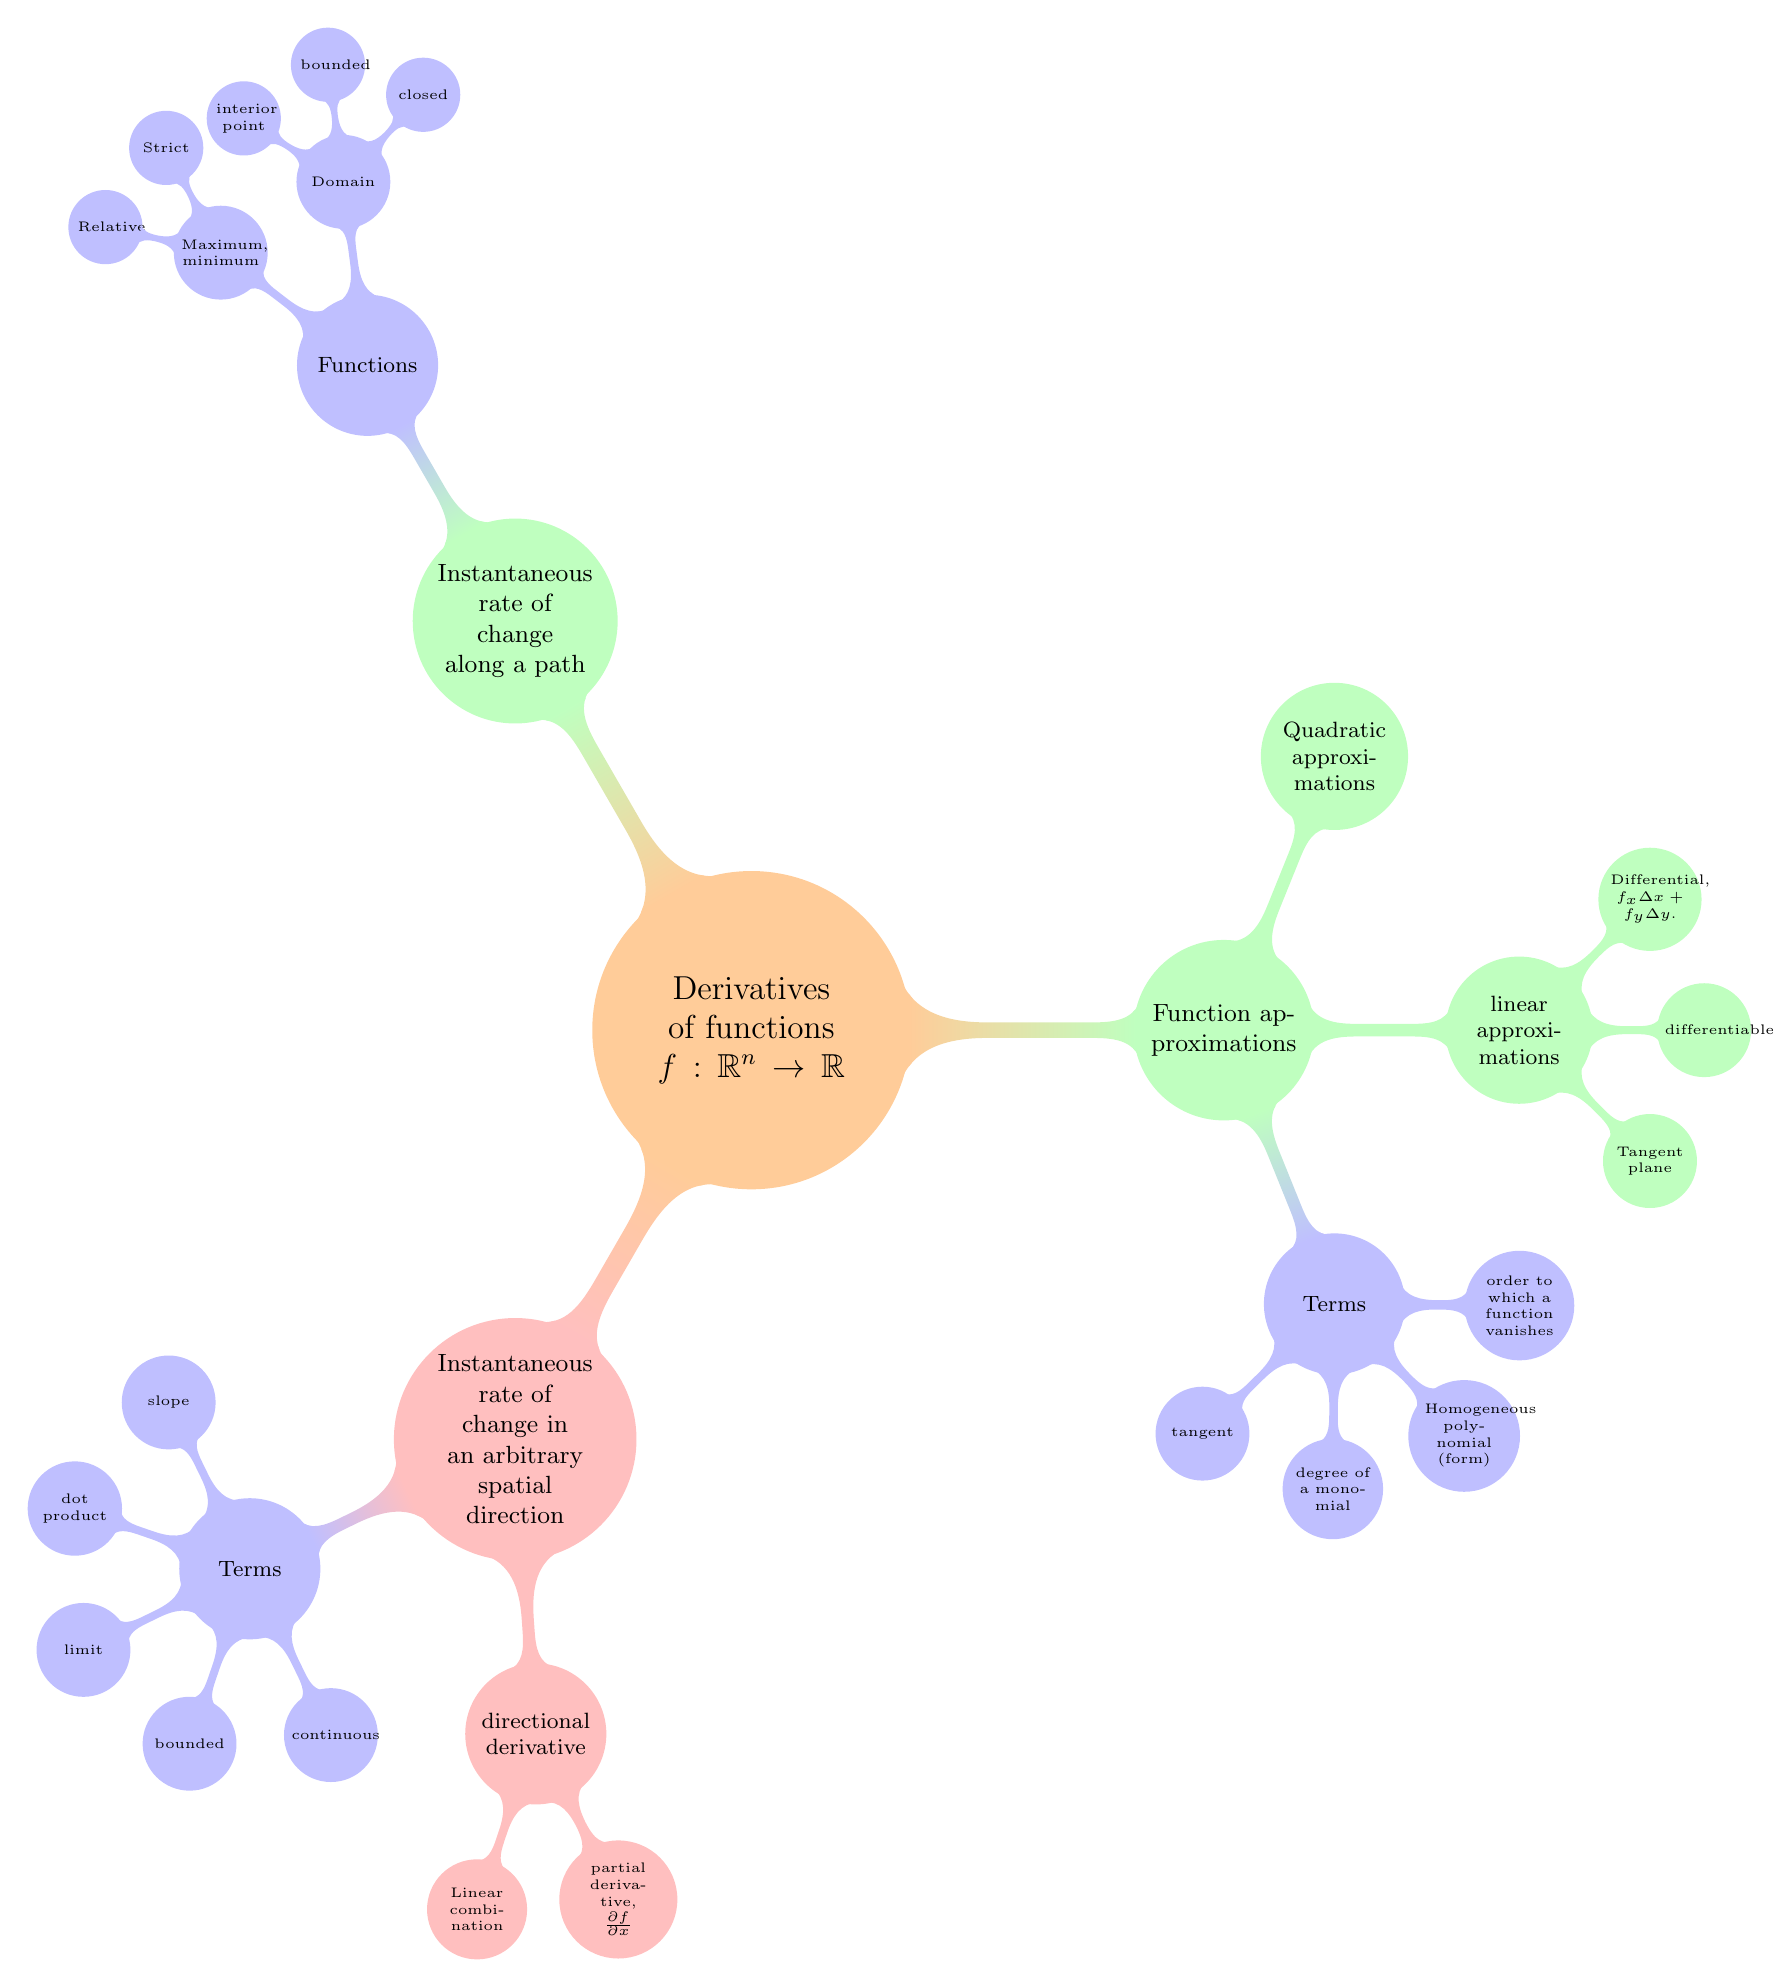
\begin{tikzpicture}[mindmap, grow cyclic, every node/.style=concept, concept color=orange!40, 
    level 1/.append style={level distance=6cm,sibling angle=120},
    level 2/.append style={level distance=3.75cm,sibling angle=68},
    level 3/.append style={level distance=2.35cm,sibling angle=45},
    level 4/.append style={level distance=1.5cm,sibling angle=50}]
    \node{Derivatives of functions $f: \mathbb{R}^n \rightarrow \mathbb{R}$}
        child[concept color=red!25] { node {Instantaneous rate of change in an arbitrary spatial direction}
          	child[concept color=blue!25]  { node {Terms}
		child { node {slope}}
		child { node {dot product}}
		child { node {\gls{limit}}}
		child { node {bounded}}
		child { node {\gls{continuous}}}
		}
		%child[concept color=blue!25] { node {Functions: Level sets}}
       	 	child { node {\gls{directional derivative}}
			child { node {Linear combination}}
			child { node {\gls{partial derivative}, $\frac{\partial f}{\partial x}$}}
		}
	}
	        child[concept color=green!25] { node {Function approximations}
        child[concept color=blue!25]  { node {Terms}
		child { node {\gls{tangent}}}
		child { node {\gls{degree} of a \gls{monomial}}}
		child { node {Homogeneous polynomial (\gls{form})}}
		child { node {\gls{order} to which a function vanishes}}
		}
	%child[concept color=blue!25] { node {Necessary vs sufficient condition}}
        	child { node {\gls{linear} approximations}
		child{ node {Tangent plane}
		}
		child { node {\gls{differentiable}}}
		child { node {Differential, $f_x \Delta x +f_y \Delta y$.}}
		}
		child { node {Quadratic approximations}}
		}
		 child[concept color=green!25] { node {Instantaneous rate of change along a path}
		 		child[concept color=blue!25] { node {Functions}
        		child[concept color=blue!25] { node {Domain}
			child { node {closed}}
			child { node {bounded}}
			child { node {interior point}}
		}
      		child[concept color=blue!25] { node {Maximum, minimum}
			child { node {Strict}}
			child { node {Relative}}
		}}
		};
\end{tikzpicture}
}

\printnoidxglossaries
% Glossary instruction:
% http://mirror.unl.edu/ctan/macros/latex/contrib/glossaries/glossariesbegin.pdf
\end{document}
